\subsection{Use case diagram}
	A global picture of the system interaction with actors is provided here by means of use case diagrams. Following, an analysis of the most interesting use case situations derived from scenarios is presented.

	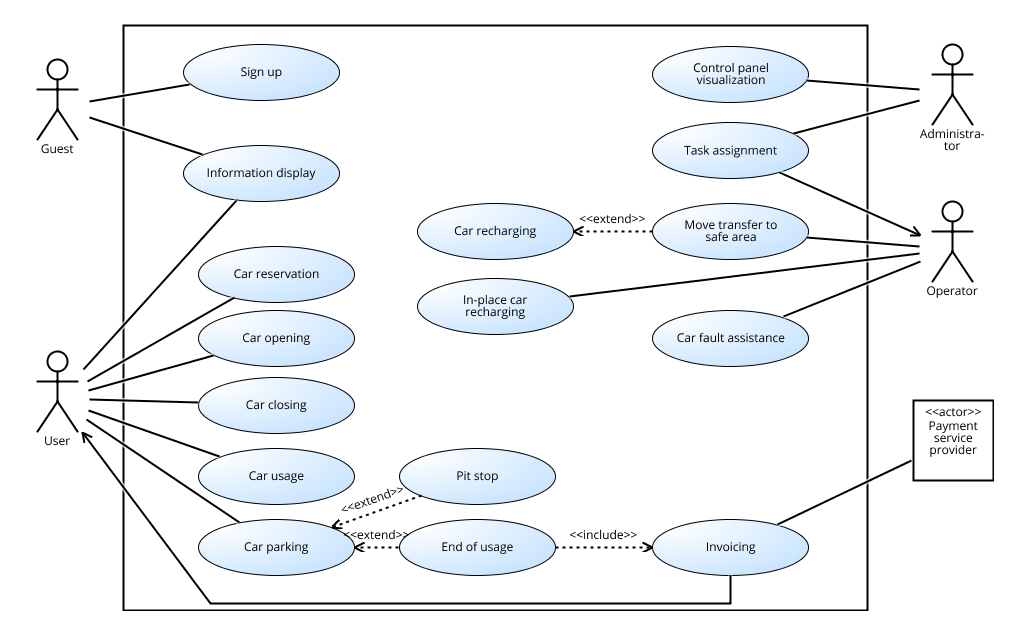
\includegraphics[width=\textwidth]{img/use_case.png}

	\subsubsection{Use case 1: Reserve a car}
		\begin{description}
			\item[Name] Reserve a car
			\item[Actors] \hfill
				\begin{description}
					\item[User] The user who wants to reserve a car.
				\end{description}
			\item[Entry condition] The user decides to reserve a car to take in the next hour.
			\item[Flow of events] \hfill
				\begin{enumerate}
					\item The user logs in into the mobile app and goes to the reservation section. \item The system automatically retrieves and displays the location of the user, but they can specify a different location if needed.
					\item The system displays the position of the available cars close to the selected location.
					\item The user selects a car and confirm the reservation.
				\end{enumerate}
			\item[Exit condition] The system reserves the car for the user.
			\item[Exceptions] \hfill
				\begin{itemize}
					\item \textbf{The system is not able to locate the user automatically.} The user is required to insert a position manually.
					\item \textbf{The system is not able to find a position inserted manually.} The user is informed and the operation is aborted.
					\item \textbf{There are no available cars.} The user is informed and the operation is aborted.
					\item \textbf{The user cancels the operation before confirming.} The reservation process is not completed and the car remains available to other users.
				\end{itemize}
			\item[Special Requirements] None.
		\end{description}

	\subsubsection{Use case 2: Park in known safe area}
		\begin{description}
			\item[Name] Park in known safe area
			\item[Actors] \hfill
				\begin{description}
					\item[User] The user of the car.
					\item[Car] The car in use.
				\end{description}
			\item[Entry condition] The user is driving and has reached their destination. They know a safe area close to the destination.
			\item[Flow of events] \hfill
				\begin{enumerate}
					\item The safe area is free and the user parks in it.
					\item As the car is turned off, the system detects it is in a safe area.
					\item The system asks the user if he wants to keep the car or to end the ride.
					\item The user selects to end the ride.
					\item The user exits the car.
					\item The system closes the car.
					\item The system charges the user for the ride.
				\end{enumerate}
			\item[Exit condition] The user leaves the car and the car becomes available to other users.
			\item[Exceptions] \hfill
				\begin{itemize}
					\item \textbf{The safe area is taken.} The user can't end their ride and this operation is aborted.
					\item \textbf{The car is badly parked.} ??? % TODO
					\item \textbf{The user selects to keep the car when prompted.} The user keeps being charged and the car is not made available for other users.
				\end{itemize}
			\item[Special Requirements] None. % TODO are there any?
		\end{description}

	\subsubsection{Use case 3: Park with money saving option}
		\begin{description}
			\item[Name] Park with money saving option
			\item[Actors] \hfill
			\begin{description}
				\item[User] The user of the car.
				\item[Car] The car in use.
			\end{description}
			\item[Entry condition] The user selects the \textit{money saving option} at some point of their ride and insert their destination.
			\item[Flow of events] \hfill
			\begin{enumerate}
				\item The system indicates the user the suggested safe area for their destination.
				\item The user parks in the suggested safe area.
				% from here, same as Use case 2:
				\item As the car is turned off, the system detects it is in a safe area.
				\item The system asks the user if he wants to keep the car or to end the ride.
				\item The user selects to end the ride.
				\item The user exits the car.
				\item The system closes the car.
				\item The system charges the user for the ride. A discount is applied for using the \textit{money saving option}.
			\end{enumerate}
			\item[Exit condition] The user leaves the car and the car becomes available to other users.
			\item[Exceptions] \hfill
			\begin{itemize}
				\item \textbf{The suggested safe area becomes taken while the user is driving.} The system selects another safe area and notifies the user of the new suggestion.
				\item \textbf{The user parks in another safe area.} The system notifies the user that they will not receive a discount. If the user decides to end the ride anyway, the system charges them without applying the \textit{money saving option} discount.
				\item \textbf{The destination of the user changes.} The user selects a new destination and the system indicates another suggestion.
				\item \textbf{The user disables the \textit{money saving option} while driving.} The suggested safe area stops being displayed and the ride continues as normal.
			\end{itemize}
			\item[Special Requirements] The \textit{money saving option} must be selected before stopping the car in a parking area. % FIXME necessary?
		\end{description}

	\subsubsection{Use case 4: Park in a recharging area}
		\begin{description}
			\item[Name] Park in a recharging area
			\item[Actors] \hfill
			\begin{description}
				\item[User] The user of the car.
				\item[Car] The car in use.
			\end{description}
			\item[Entry condition] The user is about to park in a recharging area.
			\item[Flow of events] \hfill
			\begin{enumerate}
				\item The user parks the car in the recharging area.
				% same as parking in safe area
				\item As the car is turned off, the system detects it is in a safe area.
				\item The system asks the user if he wants to keep the car or to end the ride.
				\item The user selects to end the ride.
				\item The user exits the car.
				\item The system closes the car.
				\item The system charges the user for the ride.
				% /same as parking in safe area
				\item The user plugs the car into the power grid through the supply point installed in the parking space.
				\item The system detects the car is recharging.
				\item The system modifies the charge applied to the user for the ride. A 30\% discount is applied to promote virtuous behaviors.
			\end{enumerate}
			\item[Exit condition] The user leaves the car and the car becomes available to other users.
			\item[Exceptions] \hfill
			\begin{itemize}
				\item \textbf{The user does not plug the car into the power grid.} The user is charged as if they parked in a safe area.
			\end{itemize}
			\item[Special Requirements] The user plugs in the car within 5 minutes from the moment they exits the car. Otherwise the discount is not applied.
		\end{description}	
		
	\subsubsection{Use case 5: Retrieve a car with user input}
		\begin{description}
			\item[Name] Retrieve a car
			\item[Actors] \hfill
			\begin{description}
				\item[User] The user of the car.
				\item[Operator] The field operator.
			\end{description}
			\item[Entry condition] The car doesn't work and the user has parked it safely somewhere on the road.
			\item[Flow of events] \hfill
			\begin{enumerate}
				\item The user checks whether the system has already notified the breakdown.
				\item The user enters the app from their smartphone and manually notifies the malfunction.
				\item The system asks the user to fill a form with the information needed.
				\item The system locates the car.
				\item The system analyses the user's form and decides how many operatos are needed
				\item The system notifies the operators of the car's location and asks them to retrieve the car.
				\item The operators drive the truck to the car's location.
				\item The operators check the car on site.
				\item The operators loads the car on the truck and drives it away to be repaired.
				\item The system notifies the user of the annulment of all charges.
				\item The system asks the user if he wants to reserve another car.
			\end{enumerate}
			\item[Exit condition] The operator brings the car in to be repaired; the user doesn't pay anything and is offered another car.
			\item[Exceptions] \hfill
			\begin{itemize}
				\item \textbf{The user fills the form with wrong information} The field operators report this as soon as they arrive at the location and alert the system. The operators decide whether to have the user pay the fare anyway (if they inconvenienced the operators for naught) or not and notify the system. The system charges the user accordingly.
				\item \textbf{There are no cars available nearby} The system alerts the user that there are no available cars in a 1km radius. The system then asks the user if they want to increase the radius of the search or to cancel it.
				\item \textbf{The system knows of the malfunction} The system already knows of the malfunction %FIXIT is this an exception???
				\item \textbf{The car isn't safely parked} The user ticks a box in the form to inform the system of the unsafe parking. The system looks for a safe place to park nearby and notifies the operators. The operators park there and reach the car on foot to check on it. If the car needs to be transported, the operators alert the local police. 
				\item \textbf{The car is impossible to reach} The operators cannot reach the car in its location. The operators notify the system. The system alerts the local police. 
			\end{itemize}
			\item[Special Requirements] The operators must reach the car in 30 minutes time at most.
		\end{description}

	\subsubsection{Use case 6: Manually assist a parked car}
	\begin{description}
		\item[Name] Manually assist a car
		\item[Actors] \hfill
			\begin{description}
				\item[Admin] The administrator who sends the operator.
				\item[Operator] The operator sent to recover the car.
				\item[Car] The car in use.
			\end{description}
		\item[Entry condition] The administrator is notified by the system that a parked car needs manual assistance.
		\item[Flow of events] \hfill
			\begin{enumerate}
				\item The admin checks the issue the system is displaying. It can be one of the following:
					\begin{itemize}
						\item the car is in a safe area without enough power charge to be used;
						\item the car is in a recharging area without the plug inserted.
					\end{itemize}
				\item The admin assigns the maintenance work to an operator.
				\item The operator accepts the assignment and the admin is notified of it.
				\item When available, the operator performs the _maintenance operation_ (see below).
				% FIXME should he notify also the beginning of the maintenance?
				\item The operator checks the assignment as completed.
			\end{enumerate}
		\item[Exit condition] The maintenance activity has been performed and the admin is notified of the completion.
		\item[Exceptions] \hfill
			\begin{itemize}
				\item \textbf{The operator cannot is not able to the maintenance.} The assignment is marked as _not completed_, the cause is inserted into the system. The admin will be notified of it and will either assign the problem to another operator or manage it without the help of the system. The assignment will be anyway closed at the end of this process.
			\end{itemize}
		\item[Special Requirements] The operator cannot refuse an assignment and always accept it within a working day. % FIXME this can't hold: what if he's sick?..
		The operator always marks the assignment as either _completed_ or _not completed_ before the end of the workday.
	\end{description}
	In the previous use case we refer to _maintenance operation_ as to one of the following:
	\begin{itemize}
		\item \textbf{Issue}: the car is in a safe area without enough power charge to be used. \textbf{Maintenance operation}: the car is towed to a recharging area and plugged into the power grid once there.
		\item \textbf{Issue}: the car is in a recharging area without the plug inserted. \textbf{Maintenance operation}: the car is plugged into the power grid.
	\end{itemize}
